\chapter{Projeto de uma ponte de concreto armado}

\section{Objetivo}

Projetar a superestrutura de uma ponte apoiada sobre duas vigas de concreto armado. O projeto
terá a mesma largura e comprimento da seção feita com CUAD da ponte Jakway Park, de modo a comparar
as características do projeto de descobrir vantagens e desvantagens acerca da escolha de cada um dos
métodos no estudo de caso.

\section{Escopo}

Normas brasileiras serão utilizadas para este dimensionamento, mas deixando claro as disparida-
des entre as normas brasileira e as normas estadunidenses, afim de tornar a comparação mais transparente.

\section{Fundamentos para um projeto de pontes}

\citeonline[p.~29, tradução nossa]{Troitsky} afirma que um projeto de pontes é um problema complexo
de engenharia, o qual envolve diversos fatores, como o sistema da ponte, materiais, dimensões, fundações,
estética, paisagem local e ambiente.

Na fase preliminar, o projetista analisa todos os fatores baseado em sua própria criatividade,
experiência, conhecimento e capacidade de inovação (a parte artística do projeto). Em seguida, ocorre o
refinamento do projeto de acordo com os aspectos econômicos e práticos que a obra exige. Depois que
todas as exigências estéticas e funcionais são definidas, parte-se para a fase final do projeto, que requer
um estudo e análise detalhada da estabilidade da ponte e seu comportamento estrutural \cite[p.~30]{Troitsky}.

Um projeto de pontes envolve uma enorme quantidade de dados e diversos outros fatores, mas
por questões de brevidade, a definição acima é suficiente para o desenvolvimento deste trabalho.

\section{Definição: pontes e obras de arte}

Primeiramente, é preciso deixar claro que pontes e obras de arte são termos intercambiáveis.
Segundo \citeonline[p.~29, tradução nossa]{Troitsky}, a caracterização de pontes como obras de arte se deve à mescla de
arte com embasamento técnico, necessários para sua concepção. Estruturalmente falando, pontes, viadutos
e passarelas possuem processos basicamente idênticos de concepção e construção. \citeonline[p.~1]{Pfeil} as
define da seguinte forma (grifo nosso):

\begin{citacao}
Denomina-se \textbf{ponte} a obra destinada a transposição de obstáculos à continui-
dade do leito normal de uma via, tais como rios, braços de mar, vales profundos,
outras vias, etc. Quando a ponte tem por objetivo a transposição de vales,
outras vias ou obstáculos em geral não constituídos por água é, comumente,
denominada \textbf{viaduto}.
\end{citacao}

A NBR 7188 \cite[p.~1, grifo do autor]{NBR7188:2013} dá a seguinte definição:

\begin{citacao}
\textbf{ponte}\\
estrutura sujeita a ação de carga em movimento com posicionamento variável,
aqui chamada de carga móvel, utilizada para transpor obstáculo natural (rio,
córrego, vale, etc.)

[...]\\
\textbf{viaduto}\\
estrutura para transpor obstáculo artificial (avenida, rodovia, etc.)

[...]\\
\textbf{passarela}\\
estrutura longilínea, destinada a transpor obstáculos naturais e/ou artificiais
exclusivamente para pedestres e/ou ciclistas.
\end{citacao}

\nomenclature[A]{OAC}{Obras de arte correntes}
\nomenclature[A]{OAE}{Obras de arte especiais}

Estas obras de arte ainda podem ser divididas em duas categorias: obras de arte correntes (OAC)
e obras de arte especiais (OAE). OAC são construções que possuem um projeto padrão, enquanto OAE
são construções cujo projeto é específico para cada caso \cite{Franca}.

\subsection{Classificação de pontes}

A depender dos critérios do observador, uma ponte pode ser classificada de diferentes maneiras \cite[p.~3]{Pfeil}. Neste trabalho essas obras de arte foram classificadas conforme a natureza do tráfego,
que pode ser rodoviária, ferroviária e rodoferroviária, além das que se destinam apenas para pedestres: as
passarelas.

\subsection{Elementos constituintes}

\citeonline[p.~1]{Pfeil} divide a ponte em três partes principais:

\begin{alineas}[label=\textbullet]
  \item \textbf{infraestrutura}: trata-se da fundação, o elemento estrutural que transmite ao solo ou rocha os esforços vindos da mesoestrutura;
  \item \textbf{mesoestrutura}: comumente são os pilares, os elementos estruturais que recebem os esforços da superestrutura;
  \item \textbf{superestrutura}: conforme a finalidade da construção, constitui a parte útil, composta de lajes, vigas principais e secundárias.
\end{alineas}

Um ponte ainda pode possuir encontros: elementos estruturais responsáveis por receber o
empuxo de aterros de acesso, evitando sua transmissão aos outros elementos da ponte. São extremamente
variáveis e não são necessários em todas as obras de arte \cite[p.~1]{Pfeil}

\begin{figure}[htb]
	\caption{\label{elementos}Vista de uma ponte mostrando seus principais elementos constituintes.}
	\begin{center}
	    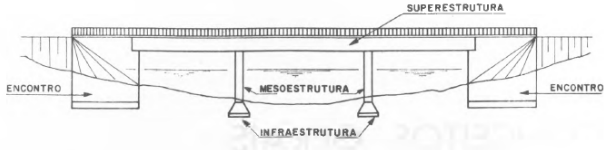
\includegraphics[max width=\textwidth]{elementos.png}
	\end{center}
	\fonte{\citeonline[p.~2]{Pfeil}}
\end{figure}

\subsection{Referências normativas}

\citeonline{DNER}, no Manual de Projeto de Obras de Arte Especiais determina o uso das seguintes normas brasileiras para o desenvolvimento de projetos de pontes (a lista foi atualizada conforme as últimas normas publicadas pela ABNT e NBR 7189, NBR 7197 e a NBR 10839 foram omitidas por terem sido canceladas e/ou substituídas):

\begin{alineas}[label=\textbullet]
  \item NBR 6118:2014 - Projeto de estruturas de concreto - Procedimento;
  \item NBR 7187:2003 - Projeto de pontes de concreto armado e de concreto protendido - Procedimento;
  \item NBR 7188:2013 - Carga móvel rodoviária e de pedestres em pontes, viadutos, passarelas e outras estruturas;
  \item NBR 7190:1997 - Projeto de estruturas de madeira;
  \item NBR 8800:2008 - Projeto de estruturas de aço e de estruturas mistas de aço e concreto de edifícios;
  \item NBR 7191:1982 - Execução de desenhos para obras de concreto simples ou armado;
  \item NBR 6122:2010 - Projeto e execução de fundações;
  \item NBR 6123:1988 - Forças devidas ao vento em edificações;
  \item NBR 6297:1983 - Levantamento geotécnico;
  \item NBR 8681:2003 - Ações e segurança nas estruturas - procedimento;
  \item NBR 9062:2017 - Projeto e execução de estruturas de concreto pré-moldado;
  \item NBR 7480:2007 - Aço destinado a armaduras para estruturas de concreto armado - Especificação;
  \item NBR 7482:2008 - Fios de aço para estruturas de concreto protendido - Especificação;
  \item NBR 7483:2008 - Cordoalhas e aço para estruturas de concreto protendido - Especificação.
\end{alineas}

\subsection{Dados necessários para um projeto de obras de arte}

Muitos dados são necessários para se projetar uma obra de arte. \citeonline[p.~19]{Leonhardt} cita alguns:

\begin{citacao}
1. Planta da situação [...];\\
2. Seção longitudinal [...];\\
3. Largura da ponte [...];\\
4. Condições das fundações [...];\\
5. Condições locais [...];\\
6. Condições meteorológicas e ambientais [...];\\
7. Estética e meio ambiente [...];\\
8. Exigências relativas ao ambiente [...].
\end{citacao}

Também é imprescindível que o projetista visite o local ou pelo menos tenha acesso a fotos de
altíssima qualidade \cite[p.~19]{Leonhardt}.

\subsection{Ações consideradas em pontes}

\nomenclature[A]{ABNT}{Associação Brasileira de Normas Técnicas}

No Brasil, os carregamentos e esforços atuantes utilizados para o projeto de pontes é fixado pela
ABNT (Associação Brasileira de Normas Técnicas). Desse modo, a NBR 7187 \cite[p.~3]{NBR7187:2013} define ações como as causas que provocam o aparecimento de esforços ou deformações nas estruturas e
as divide em três categorias:

\begin{alineas}
  \item  permanentes;
  \item  variáveis;
  \item  excepcionais.
\end{alineas}

\apudonline[p.~36]{Mason}{Hoss} lista as principais ações a que uma ponte é solicitada:

\begin{citacao}
a) Carga permanente. É avaliada com base no peso específico do concreto armado ou protendido, [...], além do peso de outros elementos, tais como pavimentação, guarda-corpos, guarda-rodas, [...];

b) Carga móvel. É fixada de acordo com o tipo de ponte e a classe de rodovia ou ferrovia. [...];

c) Impacto vertical e impacto lateral. As cargas móveis produzem efeitos dinâmicos diversos, em consequência de sua própria mobilidade, irregularidades da pista, etc.;

d) Força longitudinal. A força longitudinal é devida à frenagem e à aceleração dos veículos ou trens sobre as pontes. [...];

e) Força centrífuga. Nas pontes em curva, a carga móvel transmite à ponte uma força centrífuga [...];

f) Vento. Incide transversalmente sobre a ponte e a carga móvel, sendo o seu efeito avaliado através de pressões por unidade de área, [...];

g) Efeitos térmicos, atrito nos apoios, empuxos, movimento das fundações, etc.

Deverão ser considerados, em cada caso, de acordo com as condições especiais
da obra.
\end{citacao}

Este trabalho visa apenas dimensionar a superestrutura da ponte, portanto só serão consideradas as
ações permanentes e móveis. As ações de empuxo, variação de temperatura, vento, frenagem e aceleração
não são levadas em conta ao se lidar com a superestrutura \cite{Andrade}.

\section{Características do concreto a ser utilizado}

\nomenclature[A]{CAA}{Classe de agressividade ambiental}

A NBR 6118 \cite[p.~17]{NBR6118:2014} estabelece o uso de quatro classes de agressividade ambiental
(CAA): fraca, moderada, forte e muito forte. A ponte deste trabalho se encaixa na CAA I, agressividade
fraca e ambiente rural, portanto o risco de deterioração da estrutura é insignificante.

A partir da definição da CAA, a NBR 6118 \cite[p.~18-20	]{NBR6118:2014} determina a relação
água/cimento do concreto a ser utilizado, bem como o cobrimento nominal da armadura. Conforme a
recomendação, esta ponte deverá utilizar um concreto com relação água/cimento $ leq $ 0,65 e f\textsubscript{ck} $ geq $ 20 MPa (concreto classe 20). Para a ponte em questão, o cobrimento nominal da laje (tabuleiro da ponte) deverá ser de 20 mm. este trabalho, opta-se por utilizar um concreto com f\textsubscript{ck} = 30 MPa (concreto classe C30). Estas
definições estão resumidas na \autoref{definicoes}.

\begin{table}[htb]
\IBGEtab{%
  \caption{Definições da construção.}
  \label{definicoes}
}{%
  \begin{tabulary}{\linewidth}{CCCC}
  \toprule
  Classe de agressividade
  ambiental                 & Relação água/cimento & Cobrimento nominal da laje (mm) & Classe do concreto \\
  \midrule \midrule
   I                        & $ \leq $ 0,65        & 20                              & C30   \\
   \bottomrule
\end{tabulary}%
}{%
  \fonte{elaborado pelo autor.}%
  %\nota{Recomenda-se o uso de água de amassamento de baixa temperatura, pré cura térmica de 2 dias e cura térmica de 24 horas a uma temperatura de 80\textsuperscript{\degree} C.}
  %\nota[Anotações]{Uma anotação adicional, que pode ser seguida de várias outras.}
  }
\end{table}

\section{Pré-dimensionamento da laje}

Para estimar a espessura da laje, \citeonline[p.~53]{Leonhardt} recomenda, primeiramente, definir o
seu índice de esbeltez. \citeonline[p.~39]{Pretti} o define como "a distância aproximada entre os pontos de
momento nulo do diagrama de momentos provocado pela carga permanente"dividido pela altura da seção
transversal. Este índice é calculado conforme a \autoref{indice-esbeltez}

\begin{equation}\label{indice-esbeltez}
I_e = \frac{\ell}{h}
\end{equation}

Onde:

$ I_e = $ índice de esbeltez;

$ \ell = $ distância aproximada entre os pontos de momento nulo do diagrama de momentos provocado pela carga permanente;

$ h = $ altura da seção transversal.

\nomenclature[S]{$ I_e $}{Índice de esbeltez}
\nomenclature[S]{$ \ell $}{Distância aproximada entre os pontos de momento nulo do diagrama de momentos provocado pela carga permanente}
\nomenclature[s]{$ h $}{Altura da seção transversal}

Para o projeto em questão, uma ponte de laje maciça bi apoiada, o valor de $ \ell $ coincide com o valor
do vão teórico. \citeonline[p.~54]{Leonhardt} recomenda que o índice de esbeltez de uma ponte de laje maciça
de concreto armado classe 45 deve variar entre 15 e 22. Considerando o índice de esbeltez máximo, a
altura de laje a ser utilizada deve ser igual a 71 cm\footnote{Resolvendo a \autoref{indice-esbeltez} para h:\\ $ h = \frac{\ell}{I_e} \rightarrow h = \frac{15,6}{22} = 0,709 $}.

\section{Ações permanentes}

A NBR 7187 \cite[p.~4]{NBR7187:2013} define ações permanentes como ``Ações cujas intensidades podem ser consideradas como constantes ao longo da vida útil da construção[, incluindo] as que crescem no tempo, tendendo a um valor limite constante''.

\nomenclature[S]{kN/m\textsuperscript{2}}{Quilonewton por metro quadrado}

Além do peso próprio da laje e da pavimentação, a NBR 7187 \cite[p.~4]{NBR7187:2013} determina que deve ser considerada uma carga adicional de 2 kN/m\textsuperscript{2}, para um futuro recapeamento. A \autoref{cargas} resume os carregamentos permanentes distribuídos da ponte.

\nomenclature[S]{kN/m\textsuperscript{2}}{Quilonewton por metro quadrado}
\nomenclature[S]{kN/m\textsuperscript{3}}{Quilonewton por metro cúbico}

\begin{table}[htb]
\IBGEtab{%
  \caption{Peso específico, espessura e carregamentos distribuídos dos elementos da ponte.}
  \label{cargas}
}{%
  \begin{tabulary}{\linewidth}{CCCC}
  \toprule
   Elemento     & Peso específico (kN/m\textsuperscript{3}) & Espessura (m) & Carregamento distribuído (kN/m\textsuperscript{2}) \\
  \midrule \midrule
   Laje         & 25 \textsuperscript{a} & 0,71                    & 17,75 \\ \midrule 
   Pavimentação & 24 \textsuperscript{b} & 0,1 \textsuperscript{c} & 2,40  \\ \midrule 
   Sobrecarga   & -                      & -                       & 2 \textsuperscript{d}     \\ \midrule 
   Total        & -                      & -                       & 22,15 \\
  \bottomrule
\end{tabulary}%
}{%
  \fonte{elaborado pelo autor.}%
  \legend{ \footnotesize
  Notas: \newline
  \textsuperscript{a} Conforme NBR 6118 \cite[p.~22]{NBR6118:2014}. \newline
  \textsuperscript{b} Conforme NBR 7187 \cite[p.~4]{NBR7187:2013}. \newline
  \textsuperscript{c} Conforme Pretti \cite[p.~103]{Pretti}. \newline
  \textsuperscript{d} Conforme NBR 7187 \cite[p.~4]{NBR7187:2013}
  }
  %\nota[Anotações]{Uma anotação adicional, que pode ser seguida de várias outras.}
  }
\end{table}
Para efeito de cálculo, considera-se que a laje é um elemento isotrópico, e suas solicitações são calculadas com a teoria elástica das lajes \citeonline[p.~41]{Pretti}. Neste trabalho, optou-se por utilizar as tabelas publicadas por \citeonline{Rusch}, de modo a se calcular os valores dos momentos fletores e esforços cortantes, já que as normas brasileiras de cargas rodoviárias adotam o mesmo carregamento das normas alemãs, para o qual as tabelas foram feitas. A partir das tabelas, podemos adquirir os maiores valores dos carregamentos em suas posições mais desfavoráveis. Para automatizar o uso das tabelas de cálculo, foi utilizado o programa \textit{freeware} T-Rüsch  \cite{Serapiao_e_Khouri}.

Para calcular os esforços permanentes através das tabelas de Rüsch, além de definir as condições de apoio, é preciso definir os valores das seguintes variáveis:

\begin{alineas}[label=\textbullet]
  \item $ \ell_x $: direção principal da placa (direção dos momentos máximos);
  \item $ \ell_y $: direção ortogonal a $ \ell_x $;
  \item a: espaçamento entre rodas do veículo de cálculo (definido na NBR 7188);
  \item t: largura da distribuição de carga do veículo de cálculo (definido na NBR 7188).
\end{alineas}

\nomenclature[S]{$ \ell_x $}{Direção principal da placa (direção dos momentos máximos)}
\nomenclature[S]{$ \ell_y $}{Direção ortogonal a $ \ell_x $}
\nomenclature[S]{a}{Espaçamento entre rodas do veículo de cálculo}
\nomenclature[S]{t}{Largura da distribuição de carga do veículo de cálculo}
\nomenclature[S]{g}{Carregamento distribuído}

E em seguida determinar as relações $ \nicefrac{\ell_y}{\ell_x} $, $ \nicefrac{\ell_x}{a} $ e $ \nicefrac{t}{a} $. A \autoref{condicoes-apoio} exibe as condições de apoio da laje em questão e a \autoref{dados-rusch} define as variáveis descritas acima.

\begin{figure}[htb]
	\caption{\label{condicoes-apoio}Condições de apoio da laje. A linha cheia informa que a borda é simplesmente apoiada; a tracejada, borda livre.}
	\begin{center}
	    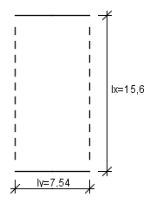
\includegraphics[max width=\textwidth]{condicoes-apoio.png}
	\end{center}
	\fonte{elaborado pelo autor}
\end{figure}

\begin{table}[htb]
\IBGEtab{%
  \caption{Definição das variáveis.}
  \label{dados-rusch}
}{%
  \begin{tabulary}{\linewidth}{CCCCC}
  \toprule
  $ \ell_x $ (m)   & $ \ell_y $ (m) &  a (m)      & t (m)        & Relações \\
  \midrule \midrule
    15,6      &  7,54      &  2      & 0,32 
   &
     $ \ell_x/\ell_y = 0,48 $
     
     $ \ell_x/a = 7,80 $
     
     $ t/a = 0,16 $ \\
  \bottomrule
  \end{tabulary}%
}{%
  \fonte{elaborado pelo autor.}%
  %\nota[Anotações]{Uma anotação adicional, que pode ser seguida de várias outras.}
  }
\end{table}

Se os valores das relações acima não existirem nas tabelas, o valor dos coeficientes é calculado por interpolação linear entre os valores disponíveis na tabela. Neste caso, o T-Rüsch faz isso automaticamente.

Por fim, o cálculo dos carregamentos permanentes é efetuado conforme a \autoref{momento} e a \autoref{cortante} \cite[adaptado]{Rusch}.

\begin{equation} \label{momento}
M = k \cdot g \cdot {\ell_x}^2
\end{equation}

\begin{equation} \label{cortante}
V = k \cdot g \cdot {\ell_x}
\end{equation}

Onde:

$ M = $ momento fletor; \\ \indent
$ V = $ esforço cortante; \\ \indent
$ k = $ coeficiente fornecido nas tabelas de Rüsch; \\ \indent
$ g = $ carregamento distribuído; \\ \indent
$ \ell_x = $ direção principal da placa (direção dos momentos máximos).

\nomenclature[S]{$ M $}{Momento fletor}
\nomenclature[S]{$ V $}{Esforço cortante}
\nomenclature[S]{$ g $}{Carregamento distribuído}
\nomenclature[S]{$ k $}{Coeficiente fornecido nas tabelas de Rüsch}

\subsection{Momentos fletores e esforços cortantes}

A \autoref{momentos-cortantes} exibe os resultados dos momentos fletores e das forças cortantes máximas resultantes das ações permanentes sobre a estrutura.


\begin{table}[htb]
\IBGEtab{%
  \caption{Momentos fletores e esforços cortantes.}
  \label{momentos-cortantes}
}{%
%\begin{tabular*}{\textwidth}{c @{\extracolsep{\fill}} ccccc}
\begin{tabulary}{1.0\textwidth}{CCCCCC}
\toprule
     & k \textsuperscript{*} & g (kN/m$^3 $) & $\ell_x (m)$ &  Resultados \\ \midrule \midrule
M\textsubscript{xm} \textsuperscript{a} & 0,125 \textsuperscript{*} &   &   & 673,80 kNm/m \\ \cmidrule{1-2}\morecmidrules \cmidrule{5-5}
M\textsubscript{ym} \textsuperscript{b} & 0,009 \textsuperscript{*} &        &  & 31,65 kNm/m \\  \cmidrule{1-2}\morecmidrules \cmidrule{5-5}
M\textsubscript{xr} \textsuperscript{c} & 0,125 \textsuperscript{*} & 22,15  & 16,6 & 673,80 kNm/m \\  \cmidrule{1-2}\morecmidrules \cmidrule{5-5}
V\textsubscript{em} \textsuperscript{d} & 0,5 \textsuperscript{**}  &      	 &  & 172,77 kN/m \\  \cmidrule{1-2}\morecmidrules \cmidrule{5-5}
V\textsubscript{er} \textsuperscript{e} & 0,5 \textsuperscript{**}  &        &  & 172,77 kN/m \\
\bottomrule
\end{tabulary} 
}{%
  \fonte{elaborado pelo autor}%
  \legend{ \footnotesize
    Notas: \newline
    \textsuperscript{a} Momento fletor da placa na direção x. \newline
    \textsuperscript{b} Momento fletor no meio da placa na direção y. \newline
    \textsuperscript{c} Momento fletor no meio dos bordos livres da placa na direção x. \newline
    \textsuperscript{d} Força cortante no meio dos apoios. \newline
    \textsuperscript{e} Força cortante no canto dos apoios. \newline
    \textsuperscript{*} Valor extraído da tabela 13 de Rüsch. \newline
    \textsuperscript{**} Valor extraído da tabela 99 de Rüsch. \newline
    \textsuperscript{***} Valor extraído da tabela 101 de Rüsch. \newline
  }
  %\nota[Anotações]{Uma anotação adicional, que pode ser seguida de várias outras.}
  }
\end{table}

\nomenclature[S]{M\textsubscript{xm}}{Momento fletor da placa na direção x}
\nomenclature[S]{M\textsubscript{ym}}{Momento fletor no meio da placa na direção y}
\nomenclature[S]{M\textsubscript{xr}}{Momento fletor no meio dos bordos livres da placa na direção x}
\nomenclature[S]{V\textsubscript{em}}{Força cortante no meio dos apoios}
\nomenclature[S]{V\textsubscript{er}}{Força cortante no canto dos apoios}

Por questões de economia e racionalização, para que se possa detalhar as armaduras, também é necessário calcular os momentos a cada décima parte do vão (neste caso, a cada 1,5 m). O valor do momento em determinada seção x da laje em estudo pode ser definido conforme a \autoref{momentos-secao}.

\begin{equation} \label{momentos-secao}
M_s = V_{max} \cdot x -\frac{g \cdot x^2}{2}
\end{equation}

Onde:

$ M_s = $ momento na seção;

$ V_{max} =  $ esforço cortante máximo;

$ g = $ carregamento distribuído.

Para fins de didáticos e de brevidade, optou-se por ignorar a contribuição de esforços provenientes das barreiras laterais, exigidas para a construção.

\section{Ações variáveis}

A NBR 7187 \cite[p.~5]{NBR7187:2013} define as ações variáveis da seguinte forma:

\begin{citacao}
Ações de caráter transitório, que compreendem, entre outras:

a) as cargas móveis;\\
b) as cargas de construção;\\
c) as cargas de vento;\\
d) o empuxo de terra provocado por cargas móveis;\\
e) a pressão da água em movimento;\\
f) o efeito dinâmico do movimento das águas;\\
g) as variações de temperatura.\\
\end{citacao}

Conforme o escopo deste trabalho, só será calculado o efeito das cargas móveis (veículos que trafegam sobre a via) sobre a laje, de acordo com as orientações da NBR 7188 \cite{NBR7188:2013}.

O cálculo da carga móvel é efetuado conforme a \autoref{carga-movel-concentrada} e a \autoref{carga-movel-distribuida}.

\begin{equation} \label{carga-movel-concentrada}
Q = P \cdot CIV \cdot CNF \cdot CIA
\end{equation}

\begin{equation} \label{carga-movel-distribuida}
q = p \cdot CIV \cdot CNF \cdot CIA
\end{equation}

Onde:

$ Q = $ carga móvel concentrada aplicada no nível do pavimento; \\ \indent
$ q = $ carga móvel estática aplicada no nível do pavimento; \\ \indent
$ P = $ carga estática aplicada no nível do pavimento; \\ \indent
$ CIV = $ coeficiente de impacto vertical; \\ \indent
$ CNF = $ coeficiente de número de faixas; \\ \indent
$ CIA = $ coeficiente de impacto adicional. \\ \indent

\nomenclature[S]{Q}{C	arga móvel concentrada aplicada no nível do pavimento}
\nomenclature[S]{q}{Carga móvel estática aplicada no nível do pavimento}
\nomenclature[S]{P}{Carga estática aplicada no nível do pavimento}
\nomenclature[S]{CIV}{Coeficiente de impacto vertical}
\nomenclature[S]{CNF}{Coeficiente de número de faixas}
\nomenclature[S]{CIA}{Coeficiente de impacto adicional}

Os coeficientes citados acima são calculados conforme a \autoref{CIV}, a \autoref{CNF} e a \autoref{CIA}.

\subsection{Coeficiente de impacto vertical}

\begin{equation} \label{CIV}
  \begin{split}
    CIV = 1,35     & \textrm{ \hspace{2em} para vãos menores que 10,0 m} \\
    CIV = 1 + 1,06 \cdot \frac{20}{Liv + 50} & \textrm{ \hspace{2em} para vãos entre 10,0 m e 200,0 m}
  \end{split}
\end{equation}

Onde:

$ Liv = $ vão da estrutura, em metros; em estruturas em balanço, é o comprimento do próprio balanço; em estruturas de vãos contínuos, é a média aritmética dos vãos.	

\subsection{Coeficiente de número de faixas}

\begin{equation} \label{CNF}
  CNF = 1 0,05 \cdot (n-2) \geq 0,9
\end{equation}

Onde:

$ n = $ número de faixas.

\subsection{Coeficiente de impacto adicional}

\begin{equation} \label{CIA}
  \begin{split}
    CIA = 1,15 & \textrm{ \hspace{2em} para obras em aço} \\
    CIA = 1,25 & \textrm{ \hspace{2em} para obras em concreto ou mistas}
  \end{split}
\end{equation}

\subsection{Carga móvel rodoviária}

A NBR 7188 \cite{NBR7188:2013} define a carga móvel rodoviária da seguinte forma:

\nomenclature[S]{kN}{Quilonewton}
\nomenclature[S]{m\textsuperscript{2}}{Metro quadrado}
\begin{citacao}
A carga móvel rodoviária padrão TB-450 é definida por um veículo tipo de 450 kN, com seis rodas P = 75 kN, três eixos de carga afastados entre si em 1,5 m, com área de ocupação de 18,0 m\textsuperscript{2}, circundada por uma carga uniformemente distribuída constante p = 5 kN/m\textsuperscript{2} [...].
\end{citacao}

A \autoref{disposicao-cargas-estaticas} ilustra o excerto acima.

\begin{figure}[htb]
	\caption{\label{disposicao-cargas-estaticas}Disposição das cargas estáticas.}
	\begin{center}
	    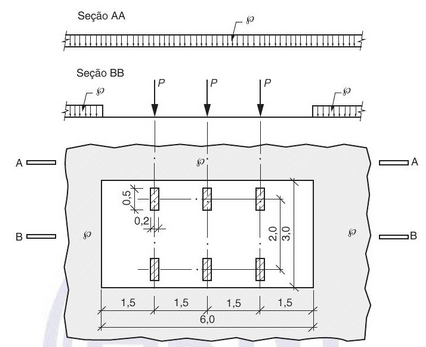
\includegraphics[max width=\textwidth]{disposicao-cargas-estaticas.png}
	\end{center}
	\fonte{NBR 7188 \cite{NBR7188:2013}}
\end{figure}

\subsection{Momentos resultantes}

Os momentos resultantes\footnote{Veja a \autoref{momentos-cortantes} para ver a qual momento cada item dos resultados se refere.} das cargas acidentais obtidos a partir do T-Rüsch são:

\nomenclature[S]{kNm/m}{Quilonewton metro por metro}

$ M_{xm} = $ 80,38 kNm/m \\ \indent
$ M_{ym} = $ 453,53 kNm/m \\ \indent
$ M_{yr} = $ 503,66 kNm/m

O memorial de cálculo gerado pelo programa T-Rüsch pode ser encontrado no \autoref{chap:memorial}